\newpage
\chapter{Fitting} \SecLabel{Fitting}

In addition to the simulation of grazing incidence
X-ray and neutron scattering by
multilayered samples, \BornAgain\ also offers the option to
fit the numerical model to reference data by modifying a selection of
sample parameters from the numerical model.  This aspect
of the software is discussed in the current chapter.

%\SecRef{FittingGentleIntroducion} gives a short introduction to the
%basic concepts of data fitting. Users familiar with fitting can
%directly proceed to \SecRef{FittingImplementation}, which details the
%implementation of fittings in 
%\BornAgain\ . 
\SecRef{FittingImplementation} details the
implementation of fittings in \BornAgain\ . 
\Python\ fitting examples with detailed
explanations of every fitting step are given in \SecRef{FittingExamples}. Advanced fitting techniques, including fine tuning of minimization
algorithms, simultaneous fit of different data sets, parameters
correlation, are covered in
\SecRef{FittingAdvanced}. \SecRef{FittingRightAnswers} contains some practical advice which might
help the user to get right answers from \BornAgain\ fitting.

%%%%%%%%%%%%%%%%%%%%%%%%%%%%%%%%%%%%%%%%%%%%%%%%%%%%%%%%%%%%%%%%%%%%%%%%%%%%%%%%
%
%%%%%%%%%%%%%%%%%%%%%%%%%%%%%%%%%%%%%%%%%%%%%%%%%%%%%%%%%%%%%%%%%%%%%%%%%%%%%%%
\section{Gentle introduction to the data fitting.} \SecLabel{FittingGentleIntroducion}

The aim of this section is to briefly introduce the basic concept of
data fitting, its key terminology and difficulties which might arise in scattering data fit.
Users wanting to find out more about minimization (also called
maximization or optimization methods depending on the formulations and objectives) 
or looking for more rigorous discussion than provided in this manual
are referred to \cite{Antoniou2007, mntutorial}

\subsection{Toy scattering experiment.}

Fig.~\ref{fig:toyfit_data},left shows scattering intensity map in arbitrary units  
as a function of (x,y) of the detector ``measured'' in toy scattering experiment.

\begin{figure}[!p]
  \centering
    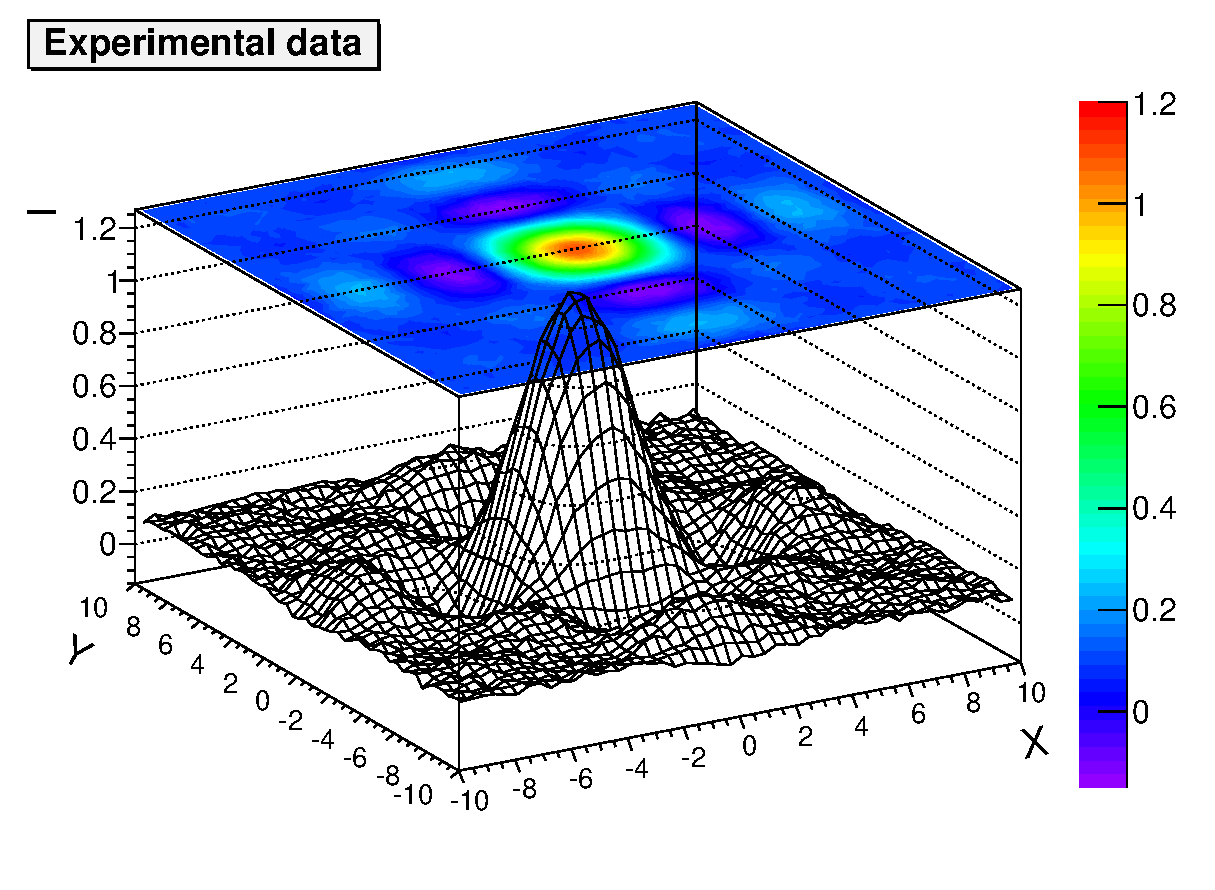
\includegraphics[width=0.49\textwidth]{Figures/toyfit_expdata.eps}
    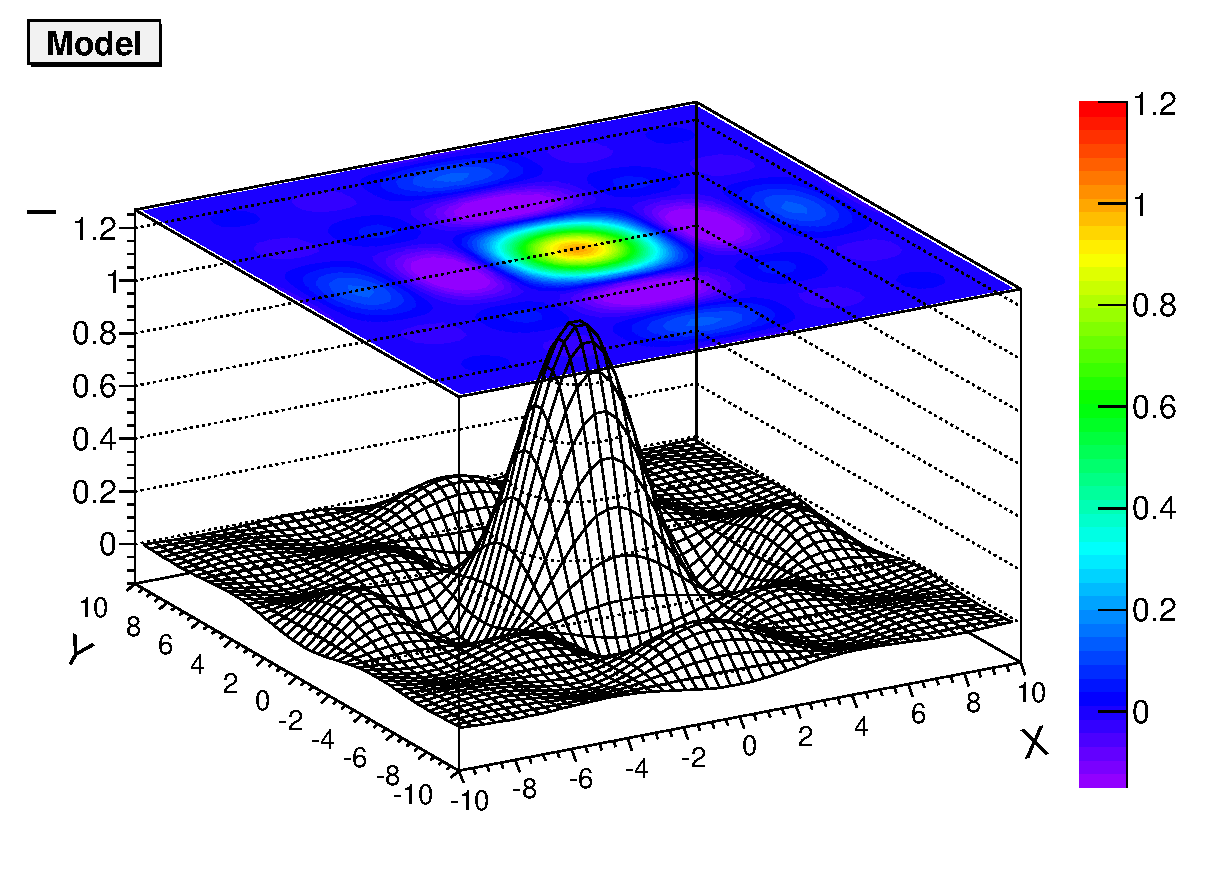
\includegraphics[width=0.49\textwidth]{Figures/toyfit_simdata.eps}
  \caption{Intensity as a function of (x,y) detector coordinates  obtained from 
  toy experiment (left) and from the toy simulation (right).   }
  \label{fig:toyfit_data}
  \vspace*{4mm}
    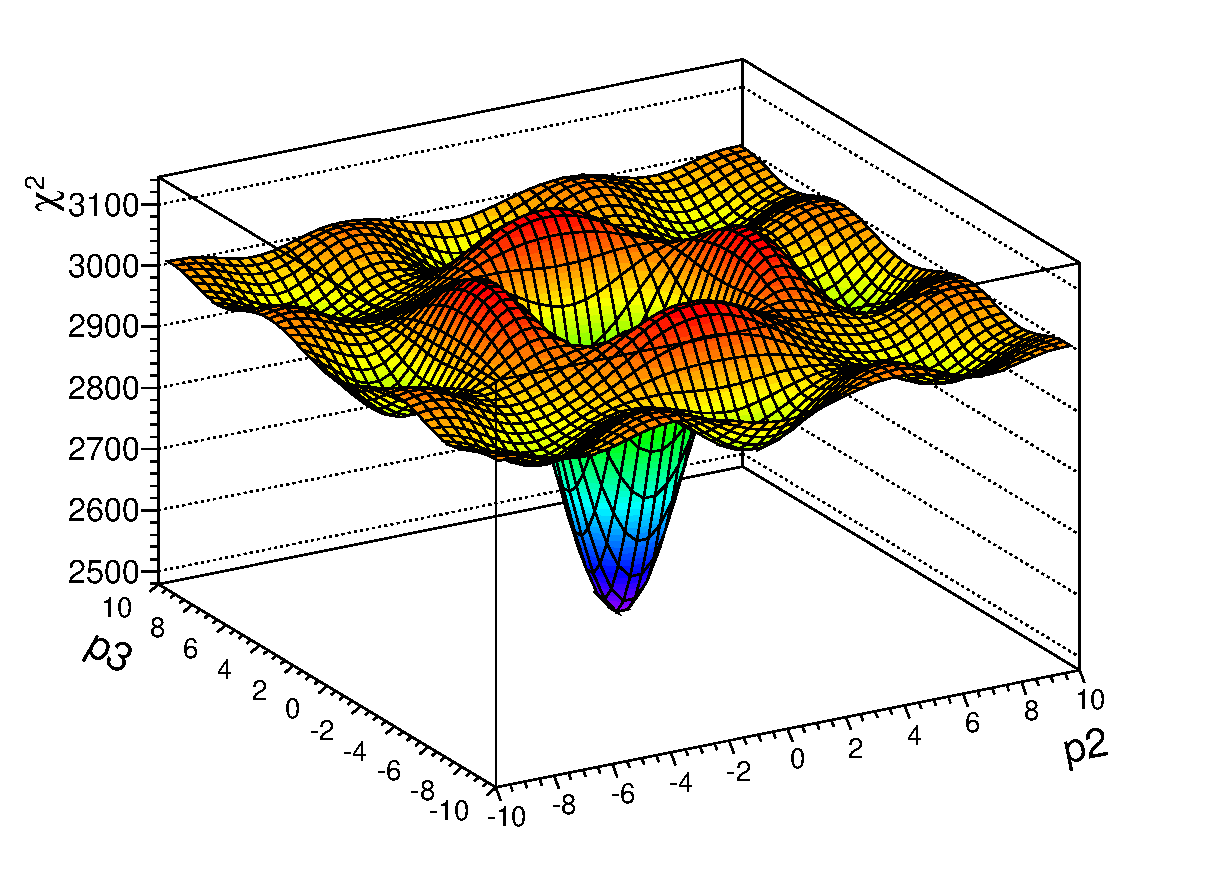
\includegraphics[width=0.49\textwidth]{Figures/toyfit_chi2_p23.eps}
    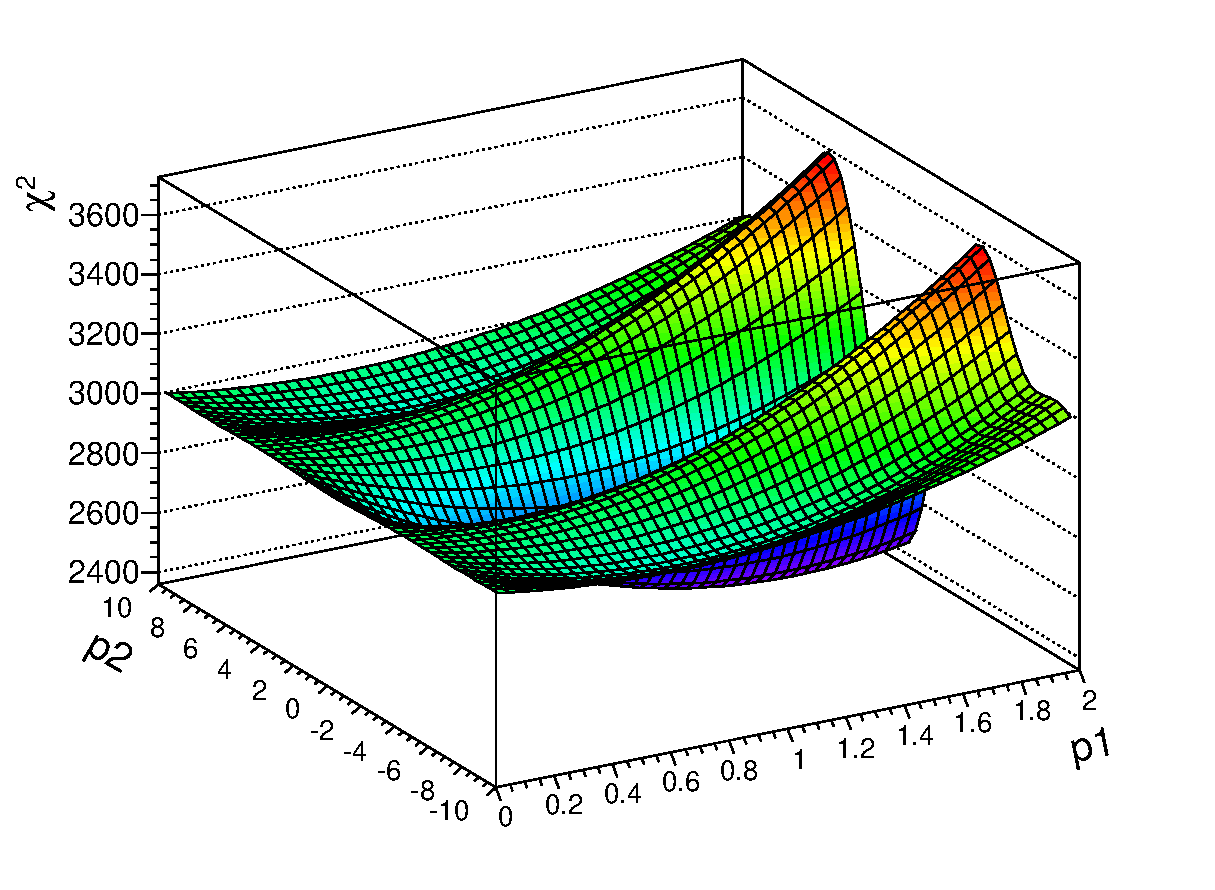
\includegraphics[width=0.49\textwidth]{Figures/toyfit_chi2_p12.eps}
  \caption{$\chi^{2}$ value calculated between experimental and simulated data
  as a function of $p_2,p_3$ parameters (left) or $p_1,p_2$ 
  parameters (right) used in the model.   }
  \label{fig:toyfit_chi2}
\end{figure}


Scattering picture presented reminds some of GISAS patterns, nevertheless it is
generated using simple function
$$I(x,y) = G(0.1,~0.01) + \frac{sin(x)}{x} \cdot \frac{sin(y)}{y}$$
Here $G(0.1, 0.01)$ is a random variable distributed according to the Gaussian distribution
with mean 0.1 and $\sigma=0.01$.
Constant $0.1$ symbolize our experimental background and constant $0.01$ is referred
to the detector noise. The rest of the formula represents our signal.

Lets define our model, namely specific mathematical function, to which we will fit our toy experimental data. By making an educated guess we assume that scattering intensity observed
in the experiment should be described with the help of $sinc$ function as follows
$$ f(x,y) = p_0 + p_1 \cdot  sinc(x - p_2) \cdot sinc(y - p_3) $$
The model has four parameters: $p_0$ describing background, $p_{1}$ describing signal strength
and $p_2,p_3$ responsible for the peak position.
Fig.~\ref{fig:toyfit_data},right shows the intensity as a function (x,y) calculated according
our model using fixed parameter set $p_0=0,p_1=1,p_2=0,p_3=0$. 

Two distributions look pretty much the same, however to find exact values of parameters which describe experimental data in the best way, one have to
\begin{itemize}
\item elaborate criteria for the difference between an actual data and its model
\item employ minimization procedure which will minimize that difference
\end{itemize}


\subsection{Objectives}

The goal is to obtain the best fit of an observed distribution
to a prediction by modifying a set of parameters from the
prediction. This problem can be one or multi-dimensional and also linear or
nonlinear. The quantity to minimize is often referred to as the
\textit{objective function}, whose expression depends on the
particular method, like the maximum likelihood, the $\chi^2$
minimization or the expected prediction error function. 

\begin{comment}
\subsubsection*{Maximum of likelihood.}
This is a popular method for parameters' estimations because the maximum likelihood estimators are approximately
unbiased and efficient for large data samples, under quite general
conditions.
We assume a sample  $\mathbf{x}=\{x_{1},x_{2},...,x_{n}\}$ of n independent and identically distributed
observations coming from probability density function $f(\mathbf{x}; \mathbf{p})$.
We assume $f(\mathbf{x}; \mathbf{p})$
to be known except for the parameters $\mathbf{p}=\{p_1,p_2,...,p_3\}$
The method of maximum likelihood takes the estimators to be
those values of $\mathbf{p}$ that maximize the likelihood function $\mathcal{L}$ as
$\mathcal{L}(\mathbf{\alpha})=\prod_{i=1}^N f(x_i;\mathbf{p})$.
Since it is easier to deal with a sum, we usually minimize
$-\text{ln}(\mathcal{L})$.
\end{comment}


\subsubsection*{$\chi^2$ or least squares minimization}
A dataset consist of $n$ data pairs $(\mathbf{x_{i}}, a_{i}), i=1,N$ where 
$\mathbf{x_{i}}$ is an independent variable and $a_{i}$ is dependent variable, whose
value is found in the measurement $i$. The number $N$ denotes the total
number of measurements. 

In the case of intensity map measured in our toy experiment 
and presented in Fig~\ref{fig:toyfit_data}, a variable $a_{i}$ denotes measured intensity, a variable $\mathbf{x_{i}}$ is a vector and correspond to the 
$(x_{i}, y_{i})$ coordinates of pixels in our detector while number $N$  corresponds 
to total number of detector pixels.

The model function has the form
$f(\mathbf{x_{i}},\mathbf{p})$
where adjustable parameters are held in the vector $\mathbf{p}$.
The least squared method finds the optimum of model function which 
fit the data in the best way by searching for the minimum of the sum of squared
residuals
$$ \chi^{2}(\mathbf{p}) = \sum_{i=1}^{N}r_{i}^{2}$$
where residual is defined as the difference between measured value and the value predicted by the model.
$$r = a_{i} - f(\mathbf{x_{i}},\mathbf{p})$$

In the case of normally distributed variables with the $\sigma^2$ variance
the quantity to minimize becomes
$$ \chi^{2}(\mathbf{p}) =
\frac{1}{d}
\sum_{i=1}^{N}  
\frac{ (a_{i} - f(\mathbf{x_{i}},\mathbf{p}))^2}{\sigma^2}   $$
where $d=N-k$ is number of degree of freedom ($k$ number of free fit parameters).


\subsubsection*{Minimization algorithms}
There are a large number of minimization algorithms providing a solution to the problem
of minimizing the objective function over the space of parameters of the function.
The minimization starts from initial guess for the parameters provided by the user,
and then evolves iteratively under control of minimization algorithm. The procedural
modifications on the parameters, the objective function, as well as convergence
criterion depend on the method implemented.
Details of particular implementation is beyond the scope of this manual and
 interested reader is encouraged to look at outside resources.



\subsubsection*{Local minima trap}




\subsection{Terminology.}

\noindent
{\bf Reference data} \\
Normally just experimental data or might be also simulated data
spoiled with the noise for purpose of testing of minimization algorithms.
\vspace*{1mm}

\noindent
{\bf Objective function} \\
Subject of minimization procedure.
\vspace*{1mm}

\noindent
{\bf Minimization} \\
Finding a best available values (i.e. local minimum) of some objective function. 
\vspace*{1mm}

\noindent
{\bf Number of degrees of freedom} \\
Number of data points - number of parameters in the fit.
\vspace*{1mm}

\noindent
{\bf Minimizer} \\
An algorithm which minimize objective function. 



%%%%%%%%%%%%%%%%%%%%%%%%%%%%%%%%%%%%%%%%%%%%%%%%%%%%%%%%%%%%%%%%%%%%%%%%%%%%%%%
%
%%%%%%%%%%%%%%%%%%%%%%%%%%%%%%%%%%%%%%%%%%%%%%%%%%%%%%%%%%%%%%%%%%%%%%%%%%%%%%%
\section{Implementation in BornAgain} \SecLabel{FittingImplementation}

Fitting in  \BornAgain\ deals with estimating the optimum parameters
in the numerical model by minimizing the difference between
numerical and reference data.
%using $\chi^2$  or maximum likelihood methods. 
The features include 

\begin{itemize}
\item a variety of multidimensional minimization algorithms and strategies.
\item the choice over possible fitting parameters, their properties and correlations.
\item the full control on objective function calculations, including applications of different normalizations and assignments of different masks and weights to different areas of reference data.
\item the possibility to fit simultaneously an arbitrary number of data sets.
\end{itemize}

Figure ~\ref{fig:minimization_workflow} shows general work flow of a typical fitting procedure.
\begin{figure}[htbp]
\centering
  \resizebox{0.99\textwidth}{!}{%
    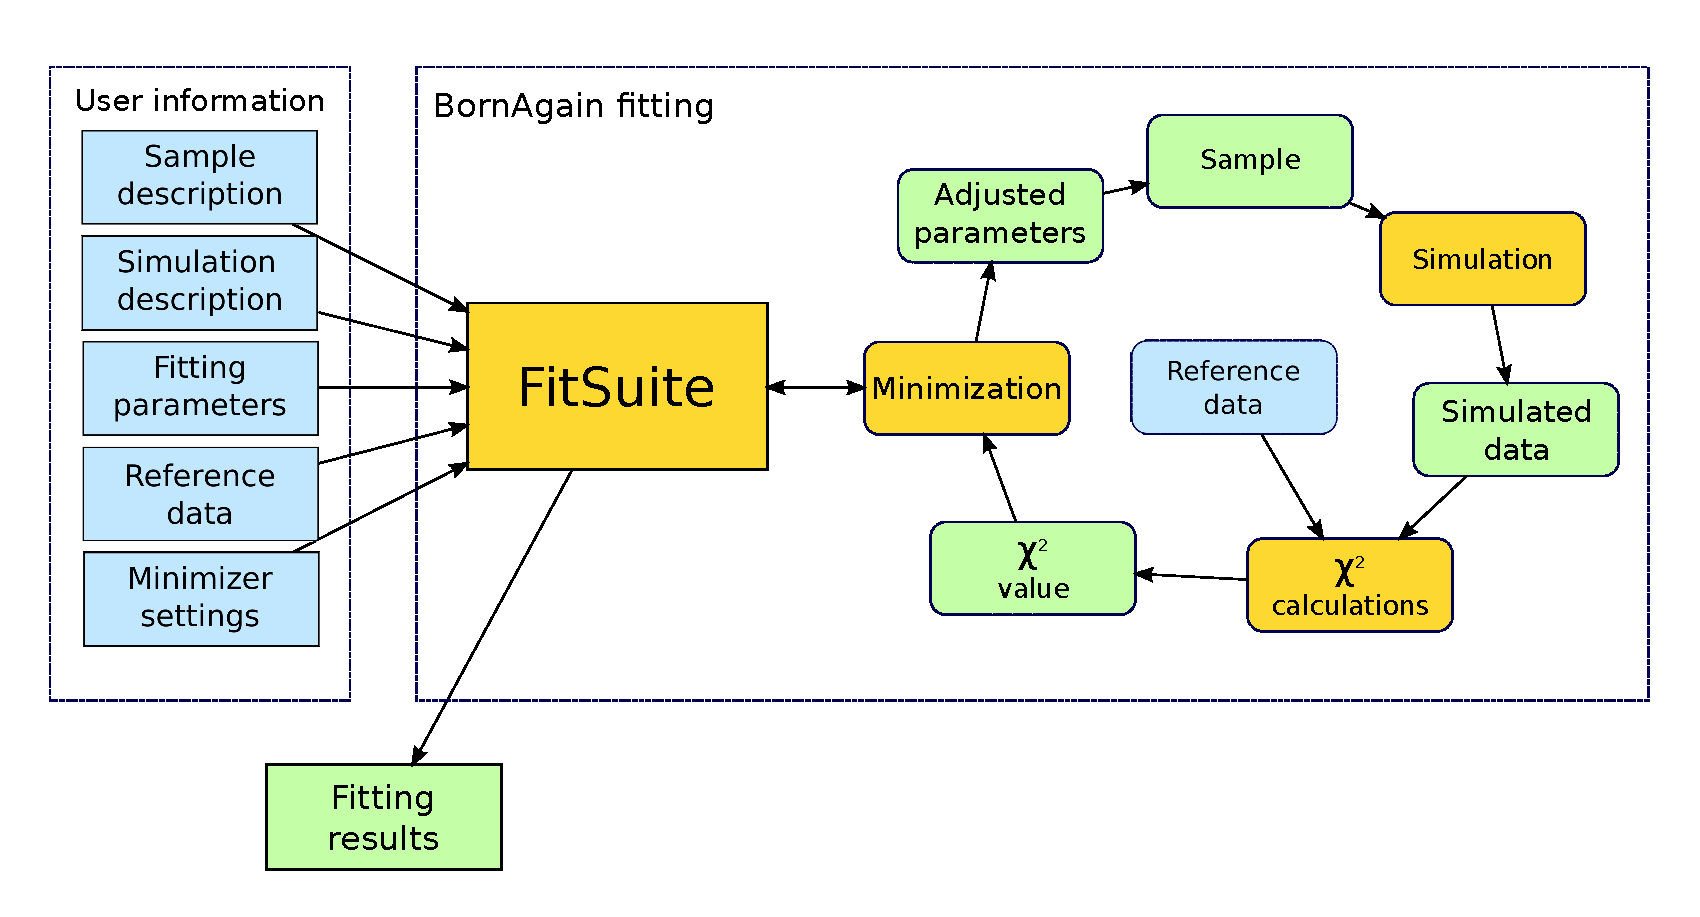
\includegraphics{Figures/minimization_workflow.eps}}
\caption{
Fitting work flow.
}
\label{fig:minimization_workflow}
\end{figure}

Before running the fitting the user is required to prepare some  data and to
configure the fitting kernel of \BornAgain\ . The required stages are

\begin{itemize}
\item Preparing the sample and the simulation description (multilayer, beam, detector parameters).
\item Choosing the fitting parameters.
\item Loading the reference data.
\item Defining the minimization settings.
\end{itemize}

The class \Code{FitSuite} contains the main functionalities to be used for the fit
and serves as the main interface between the user and the fitting work flow. 
The later involves iterations during which

\begin{itemize}
\item The minimizer makes an assumption about the optimal sample parameters.
\item These parameters are propagated to the sample.
\item The simulation is performed for the given state of the sample.
\item The simulated data (intensities) are propagated to the $\chi^2$ module.
\item The later calculates $\chi^2$ using the simulated and reference data.
\item The value of $\chi^2$ is propagated to the minimizer, which makes new assumptions about optimal sample parameters.
\end{itemize}

The iteration process is going on under the control of the selected minimization
algorithm, without any intervention from the
user. It stops 
\begin{itemize}
\item when the maximum number of iteration steps has been exceeded,
\item when the function's minimum has been reached within the tolerance window,
\item if the minimizer could not improve the values of the parameters. 
\end{itemize}

After the control is returned, fitting results can be retrieved.
They consist in the best $\chi^2$ value found, the corresponding
optimal sample parameters and the intensity map simulated with this set of parameters.

Details of \Code{FitSuite} class implementation and description
of each interface are given in \SecRef{FitSuiteClass}. The following parts of this section will detail each of
the main stages necessary to run a fitting procedure.


%%%%%%%%%%%%%%%%%%%%%%%%%%%%%%%%%%%%%%%%%%%%%%%%%%%%%%%%%%%%%%%%%%%%%%%%%%%%%%%
%
%%%%%%%%%%%%%%%%%%%%%%%%%%%%%%%%%%%%%%%%%%%%%%%%%%%%%%%%%%%%%%%%%%%%%%%%%%%%%%%
\subsection{Preparing the sample and the simulation description}

This step is similar for any simulation using \BornAgain\ (see \SecRef{Simulation}). It consists in first characterizing  the geometry of the system: the particles 
(shapes, sizes, refractive
indices), the different layers (thickness,
order, refractive index, a possible roughness of the interface), the
interference between the particles and the way they are distributed in
the layers (buried particles or particles sitting on top of a
layer). 
Then we specify the parameters of the input beam and of the
output detector.


%%%%%%%%%%%%%%%%%%%%%%%%%%%%%%%%%%%%%%%%%%%%%%%%%%%%%%%%%%%%%%%%%%%%%%%%%%%%%%%
%
%%%%%%%%%%%%%%%%%%%%%%%%%%%%%%%%%%%%%%%%%%%%%%%%%%%%%%%%%%%%%%%%%%%%%%%%%%%%%%%
\subsection{Choice of parameters to be fitted}
In principle, every parameter used in the construction of the sample
can be used as a fitting parameter. For example, the particles'
heights, radii or the layer's roughness or thickness could be selected
using the 
parameter pool mechanism. 
This mechanism is explained in detail in
\SecRef{WorkingWithSampleParameters} and it is therefore recommended
to read it before proceeding any further.

The user specifies selected sample parameters as fit parameters using \Code{FitSuite}
and its \Code{addFitParameter} method
\begin{lstlisting}[language=shell, style=commandline]
fit_suite = FitSuite()
fit_suite.addFitParameter(<name>, <initial value>, <step>, <limits>)
\end{lstlisting}
where \Code{<name>} corresponds to the parameter name in the sample's parameter pool.
By using wildcards in the parameter name, a group of sample parameters, corresponding to the given
pattern, can be associated with a single fitting parameter and 
fitted simultaneously to get a common optimal value (see \SecRef{WorkingWithSampleParameters}).

The second parameter \Code <initial value> correspond to the initial value of
the fitting parameter, while the third one
is responsible to the initial iteration steps size.
The last parameter \Code{<AttLimits>} corresponds to
the boundaries imposed on parameter value. It can be
\begin{itemize}
\item \Code{limitless()} by default, 
\item \Code{fixed()}, 
\item \Code{lowerLimited(<min\_value>)}, 
\item \Code{upperLimited(<max\_value>)}, 
\item \Code{limited(<min\_value>, <max\_value>)}.
\end{itemize}
where \Code{<min\_value>} and \Code{<max\_value>} are
double values corresponding to the lower and higher boundary, respectively.


%%%%%%%%%%%%%%%%%%%%%%%%%%%%%%%%%%%%%%%%%%%%%%%%%%%%%%%%%%%%%%%%%%%%%%%%%%%%%%%
%
%%%%%%%%%%%%%%%%%%%%%%%%%%%%%%%%%%%%%%%%%%%%%%%%%%%%%%%%%%%%%%%%%%%%%%%%%%%%%%%
\subsection{Associating reference and simulated data}

The minimization procedure deals with a pair of reference data (normally
associated with experimental data) and the theoretical model (presented by the sample and the simulation descriptions).

We assume that the experimental data are a two-dimensional intensity 
matrix as function of the output scattering
angles $\alpha_f$ and $\phi_f$ (see Fig.~\ref{fig:multil3d}).
The user is required to provide the data in the form of an ASCII file
containing an axes
binning description and the intensity data itself. 
\vspace*{2mm}

\ImportantPoint{Remark:}{
We recognize the importance of supporting the most common data formats. We are going to provide
this feature in the following releases and welcome users' requests on this subject.
}
\vspace*{1mm}

To associate the simulation and the reference data to the fitting engine, method \newline
\Code{addSimulationAndRealData} has to be used as shown
\begin{lstlisting}[language=python, style=eclipseboxed,numbers=none]
fit_suite = FitSuite()
fit_suite.addSimulationAndRealData(<simulation>, <reference>, <chi2_module>)
\end{lstlisting}

Here \Code{<simulation>} corresponds to a \BornAgain\ simulation object
with the  sample, beam and detector fully defined, \Code{<reference>}
corresponds to the experimental data object obtained from the ASCII file and \Code{<chi2\_module>} is an optional parameter for advanced 
control of $\chi2$ calculations.

It is possible to call this given method more than once to submit more than one pair of
\Code{<simulation>, <reference>} to the fitting procedure.
In this way, simultaneous fits of
some combined data sets are performed.

By using the third \Code{<chi2\_module>} parameter, different normalizations and weights
can be applied to give user full control of the way $\chi2$ is calculated.
This feature will be explained in \SecRef{FittingAdvanced}.


%%%%%%%%%%%%%%%%%%%%%%%%%%%%%%%%%%%%%%%%%%%%%%%%%%%%%%%%%%%%%%%%%%%%%%%%%%%%%%%
%
%%%%%%%%%%%%%%%%%%%%%%%%%%%%%%%%%%%%%%%%%%%%%%%%%%%%%%%%%%%%%%%%%%%%%%%%%%%%%%%
\subsection{Minimizer settings}

\BornAgain\ contains a variety of minimization engines from \Code{ROOT} and \Code{GSL}
libraries. They are listed in Table~\ref{table:fit_minimizers}.
By default \Code{Minuit2} minimizer with default settings will be used and no additional
configuration needs to be done.
The remainder of this section explains some of the expert settings, which can be applied to get better 
fit results.

The default minimization algorithm can be changed using 
\Code{MinimizerFactory} as shown below
\begin{lstlisting}[language=python, style=eclipseboxed,numbers=none]
fit_suite = FitSuite()
minimizer = MinimizerFactory.createMinimizer("<Minimizer name>","<algorithm>")
fit_suite.setMinimizer(minimizer)
\end{lstlisting}

where \Code{<Minimizer name>} and \Code{<algorithm>} can be chosen from the first and
second column of Table~\ref{table:fit_minimizers} respectively. 
The list of minimization algorithms implemented in \BornAgain\
can also be obtained using \Code{MinimizerFactory.printCatalogue()} command.


\begin{table}[h]
\centering
\begin{tabular}{@{}lll@{}}
\hline
\hline
\textbf{Minimizer name} & \textbf{Algorithm} & \textbf{Description}\\
\hline
\Code{Minuit2} \cite{MinuitURL} & \Code{Migrad} & According to
\cite{mntutorial} best minimizer for nearly all functions,\\
 & & variable-metric method with inexact line search, \\
 & & a stable metric updating scheme,\\
 & &  and checks for positive-definiteness.\\
\hline
                                       & \Code{Simplex} & simplex method of
                                       Nelder and Mead\\ 
 & & usually slower than \Code{Migrad}, \\
 &  & rather robust with respect to gross fluctuations in the\\ & &  function
 value, gives no reliable information about \\ & &  parameter errors, \\
\hline
                                       & \Code{Combined} & minimization with
                                       \Code{Migrad} \\
                                       & & but switches to Simplex if
                                       Migrad fails to converge.\\
\hline
                                       & \Code{Scan} &  not intended to
                                       minimize, just scans the
                                       function,\\
                                       & &  one parameter at a
                                       time, retains the best value
                                       after\\ &  & each scan\\
\hline
                                       & \Code{Fumili} & optimized
                                       method for least square and log
                                       likelihood\\ & &  minimizations \\
\hline
\Code{GSLMultiMin} \cite{GSLMultiMinURL} & \Code{ConjugateFR} & Fletcher-Reeves conjugate gradient
  algorithm,\\
\hline
& \Code{ConjugatePR} & Polak-Ribiere conjugate gradient algorithm,\\ 
\hline
& \Code{BFGS} & Broyden-Fletcher-Goldfarb-Shanno algorithm,\\ 
\hline
& \Code{BFGS2} & improved version of BFGS,\\ 
\hline
& \Code{SteepestDescent} & follows the downhill gradient of the function at each step\\
\hline
\Code{GSLMultiFit} \cite{GSLMultiFitURL} & & Levenberg-Marquardt
Algorithm\\
\hline
\Code{GSLSimAn} \cite{GSLSimAnURL}& & Simulated Annealing Algorithm\\ 
\hline
\hline
\end{tabular}
\caption{List of minimizers implemented in \BornAgain. }
\label{table:fit_minimizers}
\end{table}

There are several options common to every minimization algorithm, which can be changed
before starting the minimization. They are handled by \Code{MinimizerOptions} class:
\begin{lstlisting}[language=python, style=eclipseboxed, numbers = none]
options = MinimizerOptions()
options.setMaxFunctionCalls(10)
fit_suite.getMinimizer().setOptions(options)
\end{lstlisting}
In the above code snippet, a number of ``maximum function calls'',
namely the maximum number of times the minimizer is allowed to call the simulation, is limited to 10. %The minimizer will take that number into consideration and will try to limit number of iterations by that value.

There are also expert-level options common for all minimizers as well
as a number of options to tune individual minimization algorithms.
They will be explained in \SecRef{FittingAdvanced}.


%%%%%%%%%%%%%%%%%%%%%%%%%%%%%%%%%%%%%%%%%%%%%%%%%%%%%%%%%%%%%%%%%%%%%%%%%%%%%%%
%
%%%%%%%%%%%%%%%%%%%%%%%%%%%%%%%%%%%%%%%%%%%%%%%%%%%%%%%%%%%%%%%%%%%%%%%%%%%%%%%
\subsection{Running the fitting ant retrieving the results}

After the initial configuration of \Code{FitSuite} has been performed, the fitting
can be started using the command
\begin{lstlisting}[language=python, style=eclipseboxed, numbers = none]
fit_suite.runFit()
\end{lstlisting}

Depending on the complexity of the sample and the number of free sample parameters the fitting
process can take from tens to thousands of iterations. The results of the fit can
be printed on the screen using the command
\begin{lstlisting}[language=python, style=eclipseboxed, numbers = none]
fit_suite.printResults()
\end{lstlisting}
\SecRef{FittingExamples} gives more details about how to access the fitting results.




\section{Basic Python fitting example} \SecLabel{FittingExamples}

In this section we are going to go through a complete example of
fitting using \BornAgain. Each  step will be associated with a
detailed piece of code written in \Python. 
The complete listing of
the script is given in Appendix (see Listing~\ref{PythonFittingExampleScript}).
The script can also be found at
\begin{lstlisting}[language=shell, style=commandline]
./Examples/python/fitting/ex002_FitCylindersAndPrisms/FitCylindersAndPrisms.py
\end{lstlisting}

\noindent
This example uses the same sample geometry as in \SecRef{Example1Python}.
Cylindrical and
prismatic particles in equal proportion are deposited on a substrate layer, with no interference
between the particles. We consider the following parameters to be unkown
\begin{itemize}
\item the radius of cylinders,
\item the height of cylinders,
\item the length of the prisms' triangular basis,
\item the height of prisms.
\end{itemize}

Our reference data are a ``noisy'' two-dimensional intensity
map obtained from the simulation of the same geometry with a fixed
value of $5\,{\rm nm}$ for the height and radius of cylinders and for the
height of prisms which have a 10-nanometer-long side length. 
Then we run our fitting using default minimizer settings
starting with a cylinder's height
of $4\,{\rm nm}$, a cylinder's radius of $6\,{\rm nm}$, 
a prism's half side of $6\,{\rm nm}$ and a height equal to $4\,{\rm nm}$.
As a result, the fitting procedure is able to find the correct value of $5\,{\rm nm}$
for all four parameters.


%%%%%%%%%%%%%%%%%%%%%%%%%%%%%%%%%%%%%%%%%%%%%%%%%%%%%%%%%%%%%%%%%%%%%%%%%%%%%%%
\subsubsection*{Importing Python libraries}
\begin{lstlisting}[language=python, style=eclipseboxed]
from libBornAgainCore import *
from libBornAgainFit import *
\end{lstlisting}
We start from importing two \BornAgain\ libraries required to create
the sample description
and to run the fitting.


%%%%%%%%%%%%%%%%%%%%%%%%%%%%%%%%%%%%%%%%%%%%%%%%%%%%%%%%%%%%%%%%%%%%%%%%%%%%%%%
\subsubsection*{Building the sample}
\begin{lstlisting}[language=python, style=eclipseboxed, firstnumber=5]
def get_sample(): @\label{script2::get_sample}@
    """
    Build the sample representing cylinders and pyramids on top of substrate without interference.
    """
    # defining materials
    m_air = HomogeneousMaterial("Air", 0.0, 0.0)
    m_substrate = HomogeneousMaterial("Substrate", 6e-6, 2e-8)
    m_particle = HomogeneousMaterial("Particle", 6e-4, 2e-8)

    # collection of particles
    cylinder_ff = FormFactorCylinder(1.0*nanometer, 1.0*nanometer)
    cylinder = Particle(m_particle, cylinder_ff)
    prism_ff = FormFactorPrism3(2.0*nanometer, 1.0*nanometer)
    prism = Particle(m_particle, prism_ff)
    particle_layout = ParticleLayout()
    particle_layout.addParticle(cylinder, 0.0, 0.5)
    particle_layout.addParticle(prism, 0.0, 0.5)
    interference = InterferenceFunctionNone()
    particle_layout.addInterferenceFunction(interference)

    # air layer with particles and substrate form multi layer
    air_layer = Layer(m_air)
    air_layer.setLayout(particle_layout)
    substrate_layer = Layer(m_substrate)
    multi_layer = MultiLayer()
    multi_layer.addLayer(air_layer)
    multi_layer.addLayer(substrate_layer)
    return multi_layer
\end{lstlisting}
The function starting at line~\ref{script2::get_sample} creates a multilayered sample
with cylinders and prisms using arbitrary $1\,{\rm nm}$ value for all size's of particles.
The details about the generation of this multilayered sample are given in \SecRef{Example1Python}.


%%%%%%%%%%%%%%%%%%%%%%%%%%%%%%%%%%%%%%%%%%%%%%%%%%%%%%%%%%%%%%%%%%%%%%%%%%%%%%%
\subsubsection*{Creating the simulation}
\begin{lstlisting}[language=python, style=eclipseboxed, firstnumber=35]
def get_simulation(): @\label{script2::get_simulation}@
    """
    Create GISAXS simulation with beam and detector defined
    """
    simulation = Simulation()
    simulation.setDetectorParameters(100, -1.0*degree, 1.0*degree, 100, 0.0*degree, 2.0*degree)
    simulation.setBeamParameters(1.0*angstrom, 0.2*degree, 0.0*degree)
    return simulation
\end{lstlisting}
The function starting at line~\ref{script2::get_simulation} creates
the simulation object with the definition of the beam and detector parameters.



%%%%%%%%%%%%%%%%%%%%%%%%%%%%%%%%%%%%%%%%%%%%%%%%%%%%%%%%%%%%%%%%%%%%%%%%%%%%%%%
\subsubsection*{Preparing the fitting pair}
\begin{lstlisting}[language=python, style=eclipseboxed, firstnumber=45]
def run_fitting(): @\label{script2::run_fitting}@
    """
    run fitting
    """
    sample = get_sample() @\label{script2::setup_simulation1}@
    simulation = get_simulation()
    simulation.setSample(sample) @\label{script2::setup_simulation2}@

    real_data = IntensityDataIOFactory.readIntensityData('refdata_fitcylinderprisms.txt') @\label{script2::real_data}@
\end{lstlisting}
Lines
~\ref{script2::setup_simulation1}-~\ref{script2::setup_simulation2}
generate the 
sample and simulation description and assign the sample to the simulation.
Our reference data are contained in the file \Code{'refdata\_fitcylinderprisms.txt'}.
 This reference had been generated by adding noise
on the scattered intensity from a numerical sample with a fixed length of 5~nm for the four fitting
parameters (\textit{i.e.} the dimensions of the cylinders and prisms).
Line ~\ref{script2::real_data} creates the real data object by loading
the ASCII data from the input file.


%%%%%%%%%%%%%%%%%%%%%%%%%%%%%%%%%%%%%%%%%%%%%%%%%%%%%%%%%%%%%%%%%%%%%%%%%%%%%%%
\subsubsection*{Setting up \rm\bf{FitSuite}}
\begin{lstlisting}[language=python, style=eclipseboxed, firstnumber=55]
    fit_suite = FitSuite() @\label{script2::fitsuite1}@
    fit_suite.addSimulationAndRealData(simulation, real_data) @\label{script2::fitsuite2}@
    fit_suite.initPrint(10) @\label{script2::fitsuite3}@
\end{lstlisting}
Line ~\ref{script2::fitsuite1} creates a \Code{FitSuite} object which provides
the main interface to the minimization kernel of \BornAgain\ . 
Line ~\ref{script2::fitsuite2} submits simulation description and real data pair to the 
subsequent fitting. Line ~\ref{script2::fitsuite3} sets up \Code{FitSuite} to print on
the screen the information about fit progress once per 10 iterations.
\begin{lstlisting}[language=python, style=eclipseboxed, firstnumber=60]
    fit_suite.addFitParameter("*FormFactorCylinder/height", 4.*nanometer, 0.01*nanometer, AttLimits.lowerLimited(0.01)) @\label{script2::fitpars1}@
    fit_suite.addFitParameter("*FormFactorCylinder/radius", 6.*nanometer, 0.01*nanometer, AttLimits.lowerLimited(0.01))
    fit_suite.addFitParameter("*FormFactorPrism3/height", 4.*nanometer, 0.01*nanometer, AttLimits.lowerLimited(0.01))
    fit_suite.addFitParameter("*FormFactorPrism3/length", 12.*nanometer, 0.02*nanometer, AttLimits.lowerLimited(0.01)) @\label{script2::fitpars2}@
\end{lstlisting}
Lines ~\ref{script2::fitpars1}--~\ref{script2::fitpars2} enter the
list of fitting parameters. Here we use the cylinders' height and
radius and the prisms' height and side length. 
The cylinder's length and prism half side are initially equal to $4\,{\rm nm}$,
whereas the cylinder's radius and the prism half side length are equal to $6\,{\rm nm}$ before the minimization. The
iteration step is equal to $0.01\,{\rm nm}$ and only the lower
boundary is imposed to be equal to $0.01\,{\rm nm}$.


%%%%%%%%%%%%%%%%%%%%%%%%%%%%%%%%%%%%%%%%%%%%%%%%%%%%%%%%%%%%%%%%%%%%%%%%%%%%%%%
\subsubsection*{Running the fit and accessing results}
\begin{lstlisting}[language=python, style=eclipseboxed, firstnumber=66]
    fit_suite.runFit() @\label{script2::fitresults1}@

    print "Fitting completed."
    fit_suite.printResults()@\label{script2::fitresults2}@
    print "chi2:", fit_suite.getMinimizer().getMinValue() 
    fitpars = fit_suite.getFitParameters()
    for i in range(0, fitpars.size()):
        print fitpars[i].getName(), fitpars[i].getValue(), fitpars[i].getError() @\label{script2::fitresults3}@
\end{lstlisting}
Line ~\ref{script2::fitresults1} shows the command to start the fitting process.
During the fitting the progress will be displayed on the screen.
Lines ~\ref{script2::fitresults2}--~\ref{script2::fitresults3} shows different ways of
accessing the fit results.


More details about fitting, access to its results and visualization of
the fit progress using matplotlib libraries can be learned from the
following detailed example
\begin{lstlisting}[language=shell, style=commandline]
./Examples/python/fitting/ex002_FitCylindersAndPrisms/FitCylindersAndPrisms_detailed.py
\end{lstlisting}



\section {Advanced fitting.} \SecLabel{FittingAdvanced}

\subsection{Affecting $\chi2$ calculations.}
\subsection{Simultaneous fit of several data sets.}
\subsection{Using fitting strategies.}
\subsection{Masking the real data.}
\subsection{Tuning fitting algorithms.}
\subsection{Fitting with correlated sample parameters.}



\section {How to get right answer from fitting.} 
\SecLabel{FittingRightAnswers}

As it was already mentioned in \SecRef{FittingGentleIntroducion}, 
one of the main difficulties in fitting the data with the model 
is the presence of multiple
local minima in the objective function. The extended list of problems causing fit to failure includes
\begin{itemize}
\item unreliable physical model
\item multiple local minima
\item unphysical behavior of objective function, unphysical regions in parameter space
\item unreliable parameter error calculation in the presence of limits on parameter value
\item often exponential behavior of objective function and corresponding numerical inaccuracies and excessive numerical roundoff in calculation of its value and derivatives
\item large correlations between parameters
\item very different scale of parameters involved in calculation
\item not positive definite error matrix even at minimum
\end{itemize}


Given list, of course, is unrelated only to \BornAgain\ fitting. It remains the same
while fitting the data with any fitting program and any kind of theoretical model.
To address all these difficulties some amount of manual tuning might be necessary. Below we give some recommendations which might help the user to achieve reliable fit results.

\subsection*{General recommendation}
\begin{itemize}
\item initially choose small number of free fitting parameters
\item eliminate redundand parameters
\item provide a good initial guess for fit parameters
\item start from default minimizer settings and turn to the fine tuning after some experience has been acquired.
\item repeat fit using different starting values for parameters or their limits
\item repeat fit fixing and releasing different groups  of parameters
\item use \Code{Minuit2} minimizer with \Code{Migrad} algorithm (default) to get most reliable parameter error estimation
\item try \Code{GSLMultiFit} minimizer or \Code{Minuit2} minimizer with \Code{Fumili} algorithm to get fewer iterations


%\subsection*{Interpretation of errors.}


{\bf to be continued... }


\end{itemize}





%%%%%%%%%%%%%%%%%%%%%%%%%%%%%%%%%%%%%%%%%%%%%%%%%%%%%%%%%%%%%%%%%%%%%%%%%%%%%%%%%%%%%
%
% Old version
%
%%%%%%%%%%%%%%%%%%%%%%%%%%%%%%%%%%%%%%%%%%%%%%%%%%%%%%%%%%%%%%%%%%%%%%%%%%%%%%%%%%%%%

\begin{comment}

\section{Short description of fitting theory}

The aim of this section is to briefly introduce the basic concept of
minimization and its key terminology. Users wanting to find out more about minimization (also called
maximization or optimization methods depending on the formulations and objectives) are referred to
\cite{Antoniou2007, mntutorial}.

\subsection{Objectives}
We generally have to obtain the best fit of an observed distribution
to a prediction by modifying a set of parameters from the
prediction. This problem can be one or multi-dimensional and also linear or
nonlinear. The quantity to minimize is often referred to as the
\textit{objective function}, whose expression depends on the
particular method, like the maximum likelihood, the $\chi^2$
minimization or the expected prediction error function. In many cases,
a number of distinct functions may need to be minimized at once, for
example, when samples are generated with respect to an independent variable (time,
position,\ldots). Minimization can be done according to different
definitions of the norm. For example, using the Euclidean norm, this process is
often called a least squares problem. Weights can also be added in
order to emphasize important points and neglect uncritical ones.\\

 
\MakeRemark{Remark:} {\begin{itemize}
\item The term ``minimizing'' means finding a \textbf{local} minimum of the objective function.
\item The number of observations must greatly exceed the number of fitting
  parameters that are to be estimated.
\end{itemize}}

We are now going to detail two methods by specifying the expression of
the function to minimize: maximum of likelihood and $\chi^2$ minimization.

\subsubsection{Maximum of likelihood}
This is a popular method for parameters' estimations because the maximum likelihood estimators are approximately
unbiased and efficient for large data samples, under quite general
conditions.
We consider a random variable $\mathbf{x}$ (it could be a vector) distributed
with a distribution function $f(\mathbf{x}; \mathbf{\alpha})$. We assume $f(\mathbf{x}; \mathbf{\alpha})$
to be known except for the parameter(s) $\mathbf{\alpha}$ (which could
be a vector as well). The expression of $f(\mathbf{x};\mathbf{\alpha})$ represents the
hypothesized probability density function for the $\mathbf{x}$ variable. Then,
by repeating the measurements $N$ times, we sample $x_1,\ldots, x_N$
values. The method of maximum likelihood takes the estimators to be
those values of $\mathbf{\alpha}$ that maximize the likelihood function $\mathcal{L}$ as
$\mathcal{L}(\mathbf{\alpha})=\prod_{i=1}^N f(x_i;\mathbf{\alpha})$.
Since it is easier to deal with a sum, we usually minimize
$-\text{ln}(\mathcal{L})$.

\subsubsection{$\chi^2$ or least squares minimization}
Given a set of observations $\{x_1, x_2, \ldots, x_n\}$, with expectation values
$\{y_1(\mathbf{\alpha}),\ldots,
y_n(\mathbf{\alpha})\}$ and covariance matrix $V$ (matrix element
written $V_{i,j}$), then the set of
parameter values $\hat{\mathbf{\alpha}}$ which minimizes the quantity:
$\chi^2=\sum_{i,j} [x_i-y_j(\mathbf{\alpha})]V_{ij}[x_j-y_j(\mathbf{\alpha})]$ is called
the Least Squares Estimate for $\mathbf{\alpha}$.

If the $x_i$ are sampled from a normal distribution, then the least
squares minimization is equivalent to the maximum likelihood method:
the set of parameters $\mathbf{\alpha}$ which maximize $\mathcal{L}$ is the
same as those which minimize $\chi^2$. In this case the expression of
$\chi^2$ becomes $\sum_{i=1} ^N
[x_i-y_i(\mathbf{\alpha})]^2/\sigma_i^2$, where $\sigma_i^2$ is the
variance on $y_i (\mathbf{\alpha})$. Even if the observations are
not normally distributed, the least
squares minimization may be useful, in particular, if the distribution is approximately normal. 


\subsection{How good is the fitting result?}
%Quantify the level of agreement between the data and a hypothesis without explicit reference to alternative hypotheses.
%Limited to $\chi^2$??
%Level of agreement

In general, a minimization process is intended to compare a reference
(experimental observations) to some predictions (numerical models)
dependent on a certain number of parameters. At the end of the
minimization procedure, the user has to determine how close the estimated parameters are to the reference ones.
The first step could be a visual check by plotting both of them. On
the quantitative side, different quantities could be evaluated. The
most common tests for goodness-of-fit are the $\chi^2$ test,
Kolmogorov test, Cramer-Smirnov-Von-Mises test, runs. \\
The reduced $\chi^2$ is defined as the final sum of the squared residuals
divided by the number of degrees of freedom (\textit{number of datapoints -
number of parameters in the fit}). The
fit can be considered as good if the reduced $\chi^2 \sim 1$. \\

\MakeRemark{Remark:}{\begin{itemize}
\item A bad fit does not necessarily produce large errors and having a
  ``too good'' goodness-of-fit usually means that something is not right: for
  example, overestimated errors or the assumption of independent data when they were in fact correlated.
\item The $\chi^2$ test does not check that the uncertainties are
  Gaussian or normally distributed; it assumes that they are Gaussian. If the observations are not normally distributed, the LSE may be
useful, in particular, if the distribution is approximately normal.
\end{itemize}
}


\subsection{Main features of the minimization algorithm}

We start with some initial guesses for the parameters. We can then
proceed in different ways in order to find the best estimates of a
local minimum of our objective function. The procedural modifications
on the parameters, the objective function, as well as the convergence
criterion depend on the method implemented. For example, the
minimization could stop if the modifications on the objective function
or on the parameters between consecutive iterative steps are lower than a given minimization tolerance.\\
The minimization algorithms can be classified into different categories:
\begin{itemize}
\item \textit{search method}: the solution is obtained by using only function
  evaluations at different points by modifying, at each iteration, the interval between which the minimum is searched for.
\item \textit{approximate method}: close to a minimum, the function to minimize is approximated to
  a polynomial. The degree of approximation might require the evaluation of gradients or Hessian matrices (matrix of second-order partial derivatives of a function) 
\end{itemize}
Many refinements and particularities as well as other algorithms'
classifications exist. For example the
minimization can be performed by using sequential search directions that keep track of the previous steps.

In addition to the objective function, there might be some
additional conditions imposed on the parameters, for example, boundary conditions imposed on some variables or some extra relations between others. In this case, the problem is
said to be a \textit{constrained minimization problem}. Constraints
make the process more technically challenging than in unconstrained situations.


\subsection{Terminology}
\begin{itemize}
\item number of degrees of freedom = number of data points - number of fitting parameters.
\item The Hessian matrix or Hessian is a square matrix of second-order partial derivatives of a function. It describes the local curvature of a function of many variables.
\end{itemize}
%%%%%%%%%%%%%%%%%%%%%%%%%%%%%%%%%%%%%%%%%%%%%%%%%%%%%% XXX
\section{Implementation in \BornAgain}

Fitting in  \BornAgain\ deals with estimating the optimum parameters
in the numerical model by minimizing the difference between
numerical and reference data using $\chi^2$  or maximum likelihood methods. These features include different multidimensional minimization
algorithms and strategies from \Code{Root} (\Code{Minuit2} and
\Code{GSL} libraries) and the choice over possible fitting
parameters. The related codes are contained
in the folder ``Fit'' (a detailed description is given in \ldots). 

%%%%%%%%%%%%%%%%%%%%%%%%%%%%%%%%%%%%%%%
\subsection{General fitting procedure}

The general fitting procedure can be split into different steps:
\begin{enumerate}
\item Creation of the sample: multilayered sample, beam, detector,
\item Choice of the parameters to fit,
\item Loading reference data,
\item Fit: \begin{itemize}
    \item linking the reference and the numerical data, 
    \item choice of a minimizing algorithm (method, weights, strategy), 
    \item running the minimization, 
    \item checking the results.
\end{itemize}
\end{enumerate}

The class \Code{FitSuite} contains the main functionalities to be used
for the fit. The following parts of this paragraph will detail each of
the main stages before applying them to an example (see paragraph~\ref{FittingExample}).

\subsubsection{Building the sample}
This step is similar for any simulation using \BornAgain. It
consists in first characterizing  the geometry of the system: the particles (shapes, sizes, refractive
indices), the different layers (thickness,
order, refractive index, a possible roughness of the interface), the
interference between the particles and the way they are distributed in
the layers (buried particles or particles sitting on top of a
layer). Then we specify the parameters of the input beam and of the
output detector.

\subsubsection{Loading reference data}
These are the data to which the fitting model will
be compared to. They usually refer to experimental data. We assume that it is a
two-dimensional intensity matrix as function of the output scattering
angles $\alpha_f$ and $\phi_f$ (see Fig.~\ref{fig:multil3d}). The user
is required to provide reduced and \textbf{normalized} data. 

\subsubsection{Choice of parameters to be fitted}
In principle, every parameter used in the construction of the sample
can be used as a fitting parameter. For example, the particles'
heights, radii or the layer's roughness or thickness could be selected. These selected parameters
  represent the variables on which the minimizer will operate.


In \BornAgain, the parameters used for the fit are specified using the
function \Code{addFitParameter} with the following list
of variables: \Code{(<name>, <value>, <step>, <AttLimits>, <error>)} where \Code{<value>}, \Code{<step>} and \Code{<error>} are double
values corresponding to the initial value of the parameter, the
iteration step (optional parameter equal to 0.01 by default) and the error respectively. By default the input value
of \Code{<error>} is 0. \Code{<AttLimits>} corresponds to
the boundaries imposed on the range of variations of the fitting
parameter's value. It can be
\begin{itemize}
\item \Code{fixed()}, 
\item \Code{lowerLimited(<min\_value>)}, 
\item \Code{limited(<min\_value>, <max\_value>)}.
\end{itemize}
where \Code{<min\_value>} and \Code{<max\_value>} are
double values corresponding to the lower and higher boundary respectively.
The unit of \Code{<AttLimits>} is identical to the one used to characterize the
parameter's \Code{<value>}.\\

\noindent \Code{<name>} is the reference to the parameter as it had been registered
using \Code{RegisterParameter}. For example, to add the beam
intensity to the list, \Code{<name>} would be
\Code{"*Beam/intensity"}. In the case of the cylindrical particles's
 height, it would become \Code{"*FormFactorCylinder/height"}.\\

\noindent If the sample contains different types of particles, the heights of different particles can be associated to two different
fitting parameters and minimized separately.\\


\MakeRemark{Hints:}{
\begin{itemize}
\item initially choose a small number of fitting
  parameters. 
\item provide a ``good'' initial guess to save time and reduce the
  risk of failure to find the minimum looked for.
\end{itemize}}

%%%%%%%%%%%%%%%%%%%%%%%%%%%%%%%%%%%%%%%
\subsubsection{Associating reference and numerical data}
The minimization procedure deals with a pair of experimental data (the
reference) and numerical data associated with function
\Code{addSimulationAndRealData}. This provides the function to minimize
using the following syntax:

\begin{lstlisting}[language=python, style=eclipse,numbers=none]
addSimulationAndRealData(<simulation>, <reference>, <chi2_module>)
\end{lstlisting}
where \Code{<chi2\_module>}, linked to the evaluation of $\chi^2$ is
optional. Its default implementation is
 $\chi^2 =(\text{simulation}-\text{reference})^2/\text{max}(\text{reference},1).$ Other
 evaluations are possible using function \\ \Code{setChiSquaredFunction} with the following parameter:
\begin{itemize}
\item \Code{SquaredFunctionWithSystematicError($\epsilon$)}  uses
   $$\chi^2=
   \frac{(\text{sim}-\text{reference})^2}{\text{max}(|\text{reference}| +
   \epsilon^2 \text{reference}^2,1)},$$ 
where $\epsilon$ gives the ratio
   of systematic errors and is
   equal to 0.08 by default,
\item \Code{SquaredFunctionWithGaussianError($\sigma$)} uses
    $$\chi^2 =\frac{(\text{simulation}-\text{reference})^2}{\sigma^2},$$ where
    $\sigma$ is reference standard error and it is equal to 0.01 by default.
\end{itemize}
\noindent By default, all datapoints have the same weight of 1. \\



The users can therefore run a series of fits by
changing this particular association between a numerical model and
some experimental observations. For example, it is possible to generate a batch of different numerical
  samples by playing with the number of layers or the shapes of
  particles in order to obtain the best fit with the experimental
  data. 
It is possible to crop and select a single specific area in the two-dimensional space but
not  several isolated parts like around, for example, intensity maxima.

%%%%%%%%%%%%%%%%%%%%%%%%%%%%%%%%%%%%%%%
\subsubsection{Choice of fitting method}

Different minimizers from \Code{Root} library can be used in \BornAgain. They are listed in
Table~\ref{table:fit_minimizers}. Users can also add their own by
implementing the appropriate definition in the \Code{Catalogue} contained in
program \Code{MinimizerFactory}.
\Code{Minuit} user's manual describes which minimizer to use in order to best
fit your data \cite{MinuitURL}. \\


\MakeRemark{}{ The list of minimizers implemented in \BornAgain\ can be printed out using the command \Code{print
    MinimizerFactory.print\_catalogue()} for example in \Code{Python}.}

\begin{table}[h]
\centering
\begin{tabular}{@{}lll@{}}
\hline
\hline
\textbf{Minimizer name} & \textbf{Algorithm} & \textbf{Description}\\
\hline
\Code{Minuit2} \cite{MinuitURL} & \Code{Migrad} & According to
\cite{mntutorial} best minimizer for nearly all functions,\\
 & & variable-metric method with inexact line search, \\
 & & a stable metric updating scheme,\\
 & &  and checks for positive-definiteness.\\
\hline
                                       & \Code{Simplex} & simplex method of
                                       Nelder and Mead\\ 
 & & usually slower than \Code{Migrad}, \\
 &  & rather robust with respect to gross fluctuations in the\\ & &  function
 value, gives no reliable information about \\ & &  parameter errors, \\
\hline
                                       & \Code{Combined} & minimization with
                                       \Code{Migrad} \\
                                       & & but switches to Simplex if
                                       Migrad fails to converge.\\
\hline
                                       & \Code{Scan} &  not intended to
                                       minimize, just scans the
                                       function,\\
                                       & &  one parameter at a
                                       time, retains the best value
                                       after\\ &  & each scan\\
\hline
                                       & \Code{Fumili} & optimized
                                       method for least square and log
                                       likelihood\\ & &  minimizations \\
\hline
\Code{GSLMultiMin} \cite{GSLMultiMinURL} & \Code{ConjugateFR} & Fletcher-Reeves conjugate gradient
  algorithm,\\
\hline
& \Code{ConjugatePR} & Polak-Ribiere conjugate gradient algorithm,\\ 
\hline
& \Code{BFGS} & Broyden-Fletcher-Goldfarb-Shanno algorithm,\\ 
\hline
& \Code{BFGS2} & improved version of BFGS,\\ 
\hline
& \Code{SteepestDescent} & follows the downhill gradient of the function at each step\\
\hline
\Code{GSLMultiFit} \cite{GSLMultiFitURL} & & Levenberg-Marquardt
Algorithm\\
\hline
\Code{GSLSimAn} \cite{GSLSimAnURL}& & Simulated Annealing Algorithm\\ 
\hline
\hline
\end{tabular}
\caption{List of fitting minimizers implemented in \BornAgain. }
\label{table:fit_minimizers}
\end{table}


A particular algorithm is selected using function
\Code{setMinimizer}, whose syntax is the following:
\begin{lstlisting}[language=python, style=eclipse,numbers=none]
setMinimizer(MinimizerFactory.createMinimizer("<Minimizer
name>","<optional algorithm>") )
\end{lstlisting}
where \Code{<Minimizer
name>} and \Code{<optional algorithm>} can be chosen from the first and
second column
of Table~\ref{table:fit_minimizers} respectively. For example the
users could select \Code{(``Minuit2'',''Migrad'')} or
\Code{(``GSLMultiFit'',"")}.

Some of these algorithms require the estimation of a gradient function associated with the function
to minimize. \textbf{\BornAgain\ implements it automatically if required}.\\
%"GSLMultiFit" or "Minuit2" with algorithm "Fumili"

\MakeRemark{Remark:}{There is no default minimizer implemented in \BornAgain.}

Four strategies have been implemented in \BornAgain\ and can be added
using the function \Code{addFitStrategy}:
\begin{itemize}
\item \Code{FitSuiteStrategyDefault} is the default fit strategy. It just lets \Code{FitSuite} run its minimization round,
\item \Code{FitSuiteStrategyAdjustData} adjusts the data before running the minimization round,
\item \Code{FitSuiteStrategyAdjustParameters} fixes fit parameters and then calls minimizer,
\item \Code{FitSuiteStrategyBootstrap} helps the minimizer get out of local minima by perturbing real data.
\end{itemize}

These strategies act on the parameters or the data and they are
therefore different from those implemented in
\Code{Minuit2} \cite{MinuitURL}, which are linked with how the
minimizer runs. These \Code{Minuit} strategies can be equal 0, 1 or 2
(default value =1). The smaller values are associated with fewer
functions calls. On the contrary the higher values are more precise. In \BornAgain\ we used the default value of 1.

%Fumili: fast gradient-descent program
%%%%%%%%%%%%%%%%%%%%%%%%%%%%%%%%%%%%%%%
\subsubsection{Outputs}
The minimization stops 
\begin{itemize}
\item when the maximum number of function calls has been exceeded, 
\item when the maximum number of iteration steps has been exceeded
\item when the function's minimum has been reached within the tolerance window 
\item if the minimizer could not improve the values of
the parameters 
\item if there had been a problem with the calculation of the
  covariance matrix.
\end{itemize}
The output of the minimization can be saved in a file or printed on
the screen using the function \Code{printResults()}. During the
fitting process, intermediate results are accessible with function \Code{initPrint(<print\_every\_nth>)}, where
\Code{<print\_every\_nth>} is the of the number of
 minimization iterations between outputs.


Special attention must be payed to the
interpretation of the errors given by \Code{Minuit2} (normalization,
reliability of the estimates determined by the minimizer, statistical
interpretations) \cite{minuitv94.1,mnerror}. According to
\Code{Minuit}'s documentation, ``the best way to be absolutely sure of the errors, is to use “independent” calculations and compare them''.


%%%%%%%%%%%%%%%%%%%%%%%%%%%%%%%%%%%%%%%%%%%%%%%%%%%%%%
\subsection{Example in Python} \label{FittingExample}
In this section we are going to go through a complete example of
fitting using \BornAgain. Each of the steps will be associated with a
detailed piece of code written in Python. In addition, the complete listing of
the script is given at the end (see Listing~\ref{script_exfit1}).\\

\noindent This example uses a simple sample geometry: cylindrical and
prismatic particles in equal proportion, in an air layer, deposited on a substrate layer, with no interference
between the particles.\\ We consider four fitting parameters: the radius and height of cylinders and the
side length and height of prisms.\\  Our reference data are a ``noisy'' two-dimensional intensity
map obtained from the simulation of the same geometry with a fixed
value of 5 nanometers for the height of both particle shapes as well
as for the radius of the cylinders and the half side length of the
prisms' triangular basis. \\ Then we run our minimization consequently
using the algorithm \Code{Migrad} from \Code{Minuit2} as the minimization engine, starting with a cylinder's height
of 4~nm, a cylinder's radius of 6~nm, a prism's half side of 6~nm
and a length equal to 4~nm.\\

\MakeRemark{Order of steps}{The stages concerned with the preparation
  of the fit (generation of the sample, characteristics of the input
  beam and output detector, loading of reference data) can be interchanged.}

%%%%%%%%%%%%%%%%%%%%%
\myparagraph{\underline{Importing Python libraries and defining parameters}}

\begin{lstlisting}[language=python, style=eclipseboxed, name=exfit,nolol]
import sys, os, numpy 
import math @\label{import_libmath}@

from libBornAgainCore import * @\label{import_corelib}@
from libBornAgainFit import * @\label{import_fitlib}@

# values we want to find
cylinder_height = 5.0*nanometer @\label{cylheightini}@
cylinder_radius = 5.0*nanometer @\label{cylradini}@
prism3_half_side = 5.0*nanometer @\label{prismhlfini}@
prism3_height = 5.0*nanometer @\label{prismheightini}@
\end{lstlisting}

Apart from the standard Python libraries, we start by importing different libraries required in order to run the script.
Lines~\ref{import_corelib} and \ref{import_fitlib} import two
\BornAgain\ libraries respectively linked with the generation of the
sample and with the fitting. Then we specify the values that our fitting parameters should be equal
to at the end of the minimization (see lines~\ref{cylheightini}-\ref{prismheightini}).

%%%%%%%%%%%%%%%%%%%%%
\myparagraph{\underline{Building the sample}}

\begin{lstlisting}[language=python, style=eclipseboxed, name=exfit,nolol]
# ----------------------------------
# create sample : cylinders and prisms in the air on substrate layer
# ----------------------------------
def buildSample(): 
    # defining materials
    mAmbience = MaterialManager.getHomogeneousMaterial("Air", 0.0, 0.0 )
    mSubstrate = MaterialManager.getHomogeneousMaterial("Substrate", 6e-6, 2e-8 )
    mParticle = MaterialManager.getHomogeneousMaterial("Particle", 6e-4, 2e-8 )
    # collection of particles
    cylinder_ff = FormFactorCylinder(cylinder_height, cylinder_radius) @\label{fit_cylff}@
    cylinder = Particle(n_particle, cylinder_ff)
    prism_ff = FormFactorPrism3(prism3_height,  prism3_half_side) @\label{fit_prismff}@
    prism = Particle(n_particle, prism_ff)
    particle_decoration = ParticleDecoration()
    particle_decoration.addParticle(cylinder, 0.0, 0.5)
    particle_decoration.addParticle(prism,0.0, 0.5)  
    interference = InterferenceFunctionNone()
    particle_decoration.addInterferenceFunction(interference)
    # air layer with particles and substrate form multi layer
    air_layer = Layer(mAmbience)
    air_layer.setDecoration(particle_decoration)
    substrate_layer = Layer(mSubstrate, 0)
    multi_layer = MultiLayer()
    multi_layer.addLayer(air_layer)
    multi_layer.addLayer(substrate_layer)
    return multi_layer
# ----------------------------------
# create sample: input beam and detector - characteristics
# ----------------------------------
def createSimulation():
    simulation = Simulation()
    simulation.setDetectorParameters(100, 0.0*degree, 2.0*degree,100 , 0.0*degree, 2.0*degree)
    simulation.setBeamParameters(1.0*angstrom, 0.2*degree, 0.0*degree)
    return simulation
\end{lstlisting}

The details about the generation of this multilayered sample and the
characterization of the input beam and detector are given in \SecRef{Example1Python}.
The only difference can be seen in lines~\ref{fit_cylff},
\ref{fit_prismff}, where in this fitting example, we have to use names
for the fitting parameters instead of numerical values.

%%%%%%%%%%%%%%%%%%%%%
\myparagraph{\underline{Loading reference data}}

\begin{lstlisting}[language=python, style=eclipseboxed, name=exfit,nolol]
def GetRealData(): 
    real_data = OutputDataIOFactory.getOutputData('refdata_fitcylinderprisms.txt') @\label{fit_input_realdata}@
    return real_data
\end{lstlisting}

Our reference data are contained in file 
\Code{'refdata\_fitcylinderprisms.txt'}. They are expressed as a
two-dimensional array of the output intensity as a function of
$\alpha_f$ and $\phi_f$ (\textit{i.e.} the two output scattering
angles). In our case this reference had been generated by adding noise
on the scattered intensity from a numerical sample with a fixed length of 5~nm of the four fitting
parameters (\textit{i.e.} the dimensions of the cylinders and prisms).
 

%%%%%%%%%%%%%%%%%%%%%
\myparagraph{\underline{Preparing the fitting pair}}

\begin{lstlisting}[language=python, style=eclipseboxed,
  name=exfit,nolol]
def run_fitting(): @\label{Fit_function_run_fitting}@
    sample = buildSample() @\label{Fit_buildsample}@
    simulation = createSimulation() @\label{Fit_createsim}@
    simulation.setSample(sample) @\label{Fit_setsample}@
    # get the reference data
    real_data = GetRealData() @\label{Fit_getrealdata}@
    # run the simulation
    simulation.runSimulation() @\label{Fit_runsim}@
    # linking reference and numerical (to be fitted) data
    fitSuite = FitSuite() 
    fitSuite.addSimulationAndRealData(simulation, real_data) @\label{Fit_addrealsimdata}@
\end{lstlisting}


Lines~\ref{Fit_buildsample}-\ref{Fit_runsim} generate the numerical
model and load the reference data. Then with the \Code{FitSuite}
class, we associate this pair with \Code{addSimulationAndRealData}
(line~\ref{Fit_addrealsimdata}).\\


\ImportantPoint{Remark:}{\Code{run\_fitting()} function (line~\ref{Fit_function_run_fitting}) is concerned
  with the complete fitting procedure: preparing the fitting pair but also
  the next states of choosing the fitting parameters, the minimizer,
  and running the fit.
Therefore in Python, there must be an indentation for the script of the next
stages. This point is made clearer at the end of this section where the
full script is displayed.}

%%%%%%%%%%%%%%%%%%%%%
\myparagraph{\underline{Choice of fitting minimizer}}

\begin{lstlisting}[language=python, style=eclipseboxed,
  name=exfit,nolol]
    fitSuite.setMinimizer( MinimizerFactory.createMinimizer("Minuit2","Migrad") )  @\label{FitMinimizer}@
\end{lstlisting}

Line~\ref{FitMinimizer} implements your choice of minimizer for the
fit using the function \Code{setMinimizer}. Several options are available in \BornAgain; they are listed in
Table~\ref{table:fit_minimizers}

%%%%%%%%%%%%%%%%%%%%%
\myparagraph{\underline{Choice of numerical parameters to be fitted}}

\begin{lstlisting}[language=python, style=eclipseboxed,
  name=exfit,nolol]
    fitSuite.addFitParameter("*FormFactorCylinder/height", 4.*nanometer, 0.01*nanometer, AttLimits.lowerLimited(0.01) ) @\label{addFitparam_cheight}@
    fitSuite.addFitParameter("*FormFactorCylinder/radius", 6.*nanometer, 0.01*nanometer, AttLimits.lowerLimited(0.01) ) @\label{addFitparam_cradius}@
    fitSuite.addFitParameter("*FormFactorPrism3/height", 4.*nanometer, 0.01*nanometer, AttLimits.lowerLimited(0.01) ) @\label{addFitparam_pheight}@
    fitSuite.addFitParameter("*FormFactorPrism3/half_side", 6.*nanometer, 0.01*nanometer, AttLimits.lowerLimited(0.01) ) @\label{addFitparam_phside}@
\end{lstlisting}

Lines~\ref{addFitparam_cheight}-\ref{addFitparam_phside} enter the
list of fitting parameters. Here we use the cylinders' height and
radius and the prisms' height and half side length. The syntax of
\Code{addFitParameter} is
\begin{lstlisting}[language=python, style=eclipse,numbers=none]
FitSuite().addFitParameter(<name>, <initial value>, <iteration step>, <limits>)
\end{lstlisting}
where \Code{<name>} is the name of the registered parameter selected
as a fitting parameter. Then we input its initial
value and the iteration step used in the minimization process. Finally
\Code{<limits>} specify the boundaries of the parameter's value. Here
the cylinder's length and prism half side are initially equal to 4~nm,
whereas the cylinder's radius and the prism length are equal to 6~nm before the minimization. The
iteration step is equal to 0.01~nm and the boundaries are imposed only
on the lower one of 0.01~nm.\\


\ImportantPoint{Order of addition of fitting parameters}{The fitting
  parameters are stored in the order they are initialized. They can be
  accessed from the array
  \Code{fitSuite.getFitParameters().getValues()} indexed from 0.}

%%%%%%%%%%%%%%%%%%%%%
\myparagraph{\underline{Running the fit}}

\begin{lstlisting}[language=python, style=eclipseboxed, name=exfit,nolol]
    # run fit 
    fitSuite.runFit()    @\label{runFit}@
    # print fit results
    fitSuite.printResults() @\label{printFitresults}@
\end{lstlisting}

Line~\ref{runFit} shows the command to start the minimization
process. For this example we chose to display the final results only
using the function \Code{printResults()} (see
line~\ref{printFitresults}). But intermediate results are accessible as
mentioned above with the command \Code{printLine(<number of
 minimization iterations between prints>)}.

%%%%%%%%%%%%%%%%%%%%%%%%%%%%%%%%%%%%%%%%%%%
After running the fit, whose script is shown in
Listing~\ref{script_exfit1}, the text given in~\ref{output_exfit1} should be displayed on your
screen (generated using \Code{PrintResults}).



\begin{lstlisting}[caption={Output of fit using Python script~\ref{script_exfit1}},language=bash,basicstyle=\small\lstfontfamily,% style=commandline,
  label=output_exfit1,captionpos=b,escapeinside={@}{@}, numbers=
  none]%,breaklines = true]
--- FitSuite::printResults --------------------------
 Chi2:1.02169224e-02    chi2.NCall:155  grad.NCall:0,0,0 (neval, ngrad, total)
-----------------------------------------------------
  MinimizerType          : Minuit2
  MinimizerAlgorithm     : Migrad
--- Options -----------------------------------------
  Strategy               : 1
  Tolerance              : 1.00000000e-02
  MaxFunctionCalls       : 10000
  MaxIterations          : 10000
  Precision              : -1.00000000e+00
  ErrorDefinition        : 1.00000000e+00 (1-chi2, 0.5 likelihood)
  ExtraOptions           : 0
--- Status ------------------------------------------ 
  Status                 : 0 'OK, valid minimum'
  IsValidError           : 0 'No detailed error validation'
  CovMatrixStatus        : 3 'full accurate'
  NCalls                 : 155
  MinValue               : 1.02162327e-02
  Edm                    : 5.29113396e-08
--- Variables ---------------------------------------
  NumberOfVariables      : 4 (free), 4 (total) 
  Errors                 : yes, see below
  Npar  Name                           Value         Error         GlobalCC      
  0    *FormFactorCylinder/height      4.999918e+00  2.127799e-01  8.620908e-01  
  1    *FormFactorCylinder/radius      4.999933e+00  9.159691e-02  8.666066e-01  
  2    *FormFactorPrism3/height        5.000522e+00  4.802199e-01  8.595439e-01  
  3    *FormFactorPrism3/half_side     5.000185e+00  2.542907e-01  8.687376e-01  
--- Correlations-------------------------------------
      1.000000e+00  -2.045230e-01 -8.420057e-01 9.493872e-02  
      -2.045230e-01 1.000000e+00  2.158473e-01  -8.497385e-01 
      -8.420057e-01 2.158473e-01  1.000000e+00  -2.047101e-01 
      9.493872e-02  -8.497385e-01 -2.047101e-01 1.000000e+00
\end{lstlisting}

The displayed output starts by giving the values of \textbf{Chi2}, % ($\frac{\sum w_i ^2 (sim - reference)^2 }{\sum w_i ^2}/Ndegfreed$),
\textbf{chi2NCall} (number of calls), \textbf{grad.NCall} (for
gradient evaluation). The expression of $\chi^2$ is 
$$\sum_{\text{nb fitting parameters}}
\Big(\frac{\text{weight}}{\text{total weight}}\Big)^2
\Big(\sum\frac{(\text{sim}-\text{ref})^2}{\text{number
    deg. freedom}}\Big),$$
\textbf{TO CHECK}
where the intensity has been normalized with respect to ...
and weight is equal to 1 by default. 

Then a \textbf{Description of minimizer} used for
this particular procedure is given with its name and the associated
algorithm.\\

\noindent \textbf{Options}:
\begin{itemize}
\item \Code{Strategy}: \Code{Minuit2} strategy, equal to 1 by default (see
  \cite{MinuitURL} page 5),
\item \Code{Tolerance} = required tolerance on the function value at the minimum,
\item \Code{MaxFunctionCalls} = maximum number of function calls above which
  the calculation will stop,
\item \Code{MaxIterations} = maximum number of iterations,
\item \Code{Precision} = precision of minimizer in the evaluation of the
  objective function (a negative value corresponds to letting the minimizer choose its default one),
\item \Code{ErrorDefinition} returns the statistical scale used for calculate
  the error. It is typically 1 for Chi2 and 0.5 for likelihood
  minimization. It is equal to 1 by default, 
\item \Code{ExtraOptions} returns 0 if no other option have been implemented.
\end{itemize}

\noindent \textbf{Status}:
\begin{itemize}
\item \Code{Status} = 
  \begin{itemize}
    \item[] \Code{0}: \Code{'OK, valid minimum'},
    \item[] \Code{1}: \Code{'Didn't converge, covariance was made pos defined'},
    \item[] \Code{2}: \Code{'Didn't converge, Hesse is invalid'},
    \item[] \Code{3}: \Code{'Didn't converge, Edm is above max'},
    \item[] \Code{4}: \Code{'Didn't converge, Reached call limit'},
    \item[] \Code{5}: \Code{'Didn't converge, Any other failure'}.
  \end{itemize}

\item  \Code{IsValidError} returns true if Minimizer has performed a
  detailed error validation (\textit{e.g.} run Hesse method for \Code{Minuit}).
\begin{itemize}
    \item[] \Code{0}: \Code{'No detailed error validation'},
    \item[] \Code{1}: \Code{'Performed detailed error validation'}.
\end{itemize}

\item \Code{CovMatrixStatus}
\begin{itemize}
    \item[] \Code{-1}: \Code{'not available (inversion failed or Hesse failed)'},
    \item[]  \Code{0}: \Code{'available but not positive defined'},
    \item[]  \Code{1}: \Code{'covariance only approximate'},
    \item[]  \Code{2}: \Code{'full matrix but forced pos def'} (\Code{pos
      def} stands for positive definite),
    \item[]  \Code{3}: \Code{'full accurate'}.
\end{itemize}
\item \Code{NCalls}: number of function calls to reach the minimum,
\item \Code{MinValue} returns minimum function value,
\item \Code{Edm} returns expected vertical distance to the
  minimum. (\Code{Edm} stands for ``expected distance to the minimum'')
\end{itemize}

\noindent \textbf{Variables}: \\
This part reports the list of fitting parameters with their
names, the values determined at the end of the minimization process,
the errors...
\begin{itemize}
\item \Code{NumberOfVariables}: number of free and total variables,
\item \Code{Errors} = \Code{yes, see below} or \Code{no access}.\\
If \Code{Errors = yes, see below}, an array is displayed. The number of lines
is equal to the number \Code{Npar} of fitting parameters \Code{Name},
the \Code{Value} 
is the one reached at the minimum, the \Code{Error} corresponds to
the errors at this minimum. \Code{GlobalCC}  returns global correlation coefficient for
parameter $i$. It is
comprised between zero and one.
\end{itemize}

\noindent \textbf{Correlations} displays the correlation matrix. Each
coefficient is defined as\\
$\text{CovMat}(i,j)/\sqrt{\text{CovMat}(i,i)\text{CovMat}(j,j)}$,
where $\text{CovMat}(a,b)$ is the element of the covariant matrix at
line $a$ and column $b$. And it is comprised between -1 and 1.\\

\MakeRemark{Remark:}{Depending on the selected minimizer and the algorithm and if a local
minimum has been found, the output
might differ as, for example, the covariant matrix is not available
for some minimizers. }



\end{comment}
%%%%%%%%%%%%%%%%%%%%%%%%%%%%%%%%%%%%%%%%%%%%%%%%%%%%%%%%%%%%%%%%%%%%%%%%%%%%%%%
%
% end of commented part
%
%%%%%%%%%%%%%%%%%%%%%%%%%%%%%%%%%%%%%%%%%%%%%%%%%%%%%%%%%%%%%%%%%%%%%%%%%%%%%%%


